
\chapter{Experimental Method}
\label{chap:experimental_method}


\section{Development of Linear Motion Platform}

A robotic linear motion platform was developed using Lego\textsuperscript{\textregistered} Mindstorms\textsuperscript{\textregistered} parts.
The platform was designed to carry a Lytro camera and a Nikon D5100 DSLR camera side-by-side as close as possible, with support for both cameras made out of Lego parts.
The motion platform consisted of a wheeled based that carried the cameras attached by a sewing thread to a drum, driven by two Mindstorms motors.
The drum was manually held in place during operation, and the Matlab RWHT NXT Toolbox \cite{rwth2007toolbox} was used to interface with the motors.

The angular velocity of the drum was manually calibrated using a stopwatch and ruler, allowing a desired velocity and linear distance to set in software.
Figure \ref{fig:motion_platform} shows the design of the linear motion platform.

\begin{figure}[h]

\centering

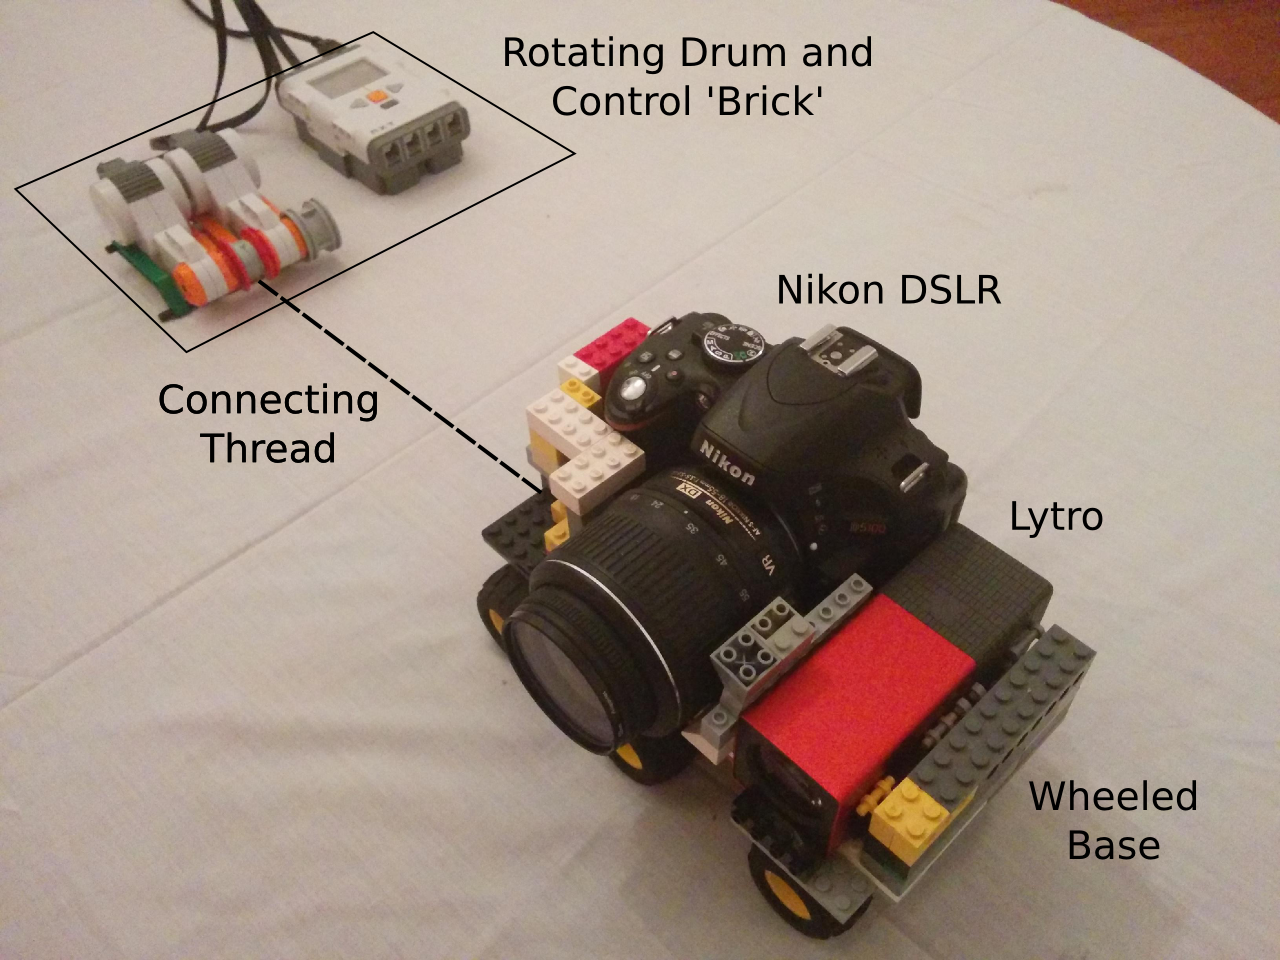
\includegraphics[width=\textwidth]{motion_platform}

\caption[Linear motion platform design]{Linear motion platform design}
\label{fig:motion_platform}

\end{figure}


\section{Scene Design}

The photographic scenes were set up in a room with no external facing windows to ensure the scene brightness could be controlled.
Three 60 watt incandescent ceiling light bulbs were used for ambient lighting and a single 72 watt diffuse incandescent desk lamp was used to provide extra light.
The desk lamp was arranged facing front-on to the scene to reduce shadow length and was placed behind the linear motion platform carrying the cameras.
A plain white sheet was placed on the working surface to reflect extra ambient light.

A large pin-board was placed behind the scene to provide a constant background depth and hardcover books were used to elevate scene elements where necessary.
Figure \ref{fig:scene_description} shows the experimental scene configuration.

\begin{figure}[h]

\centering

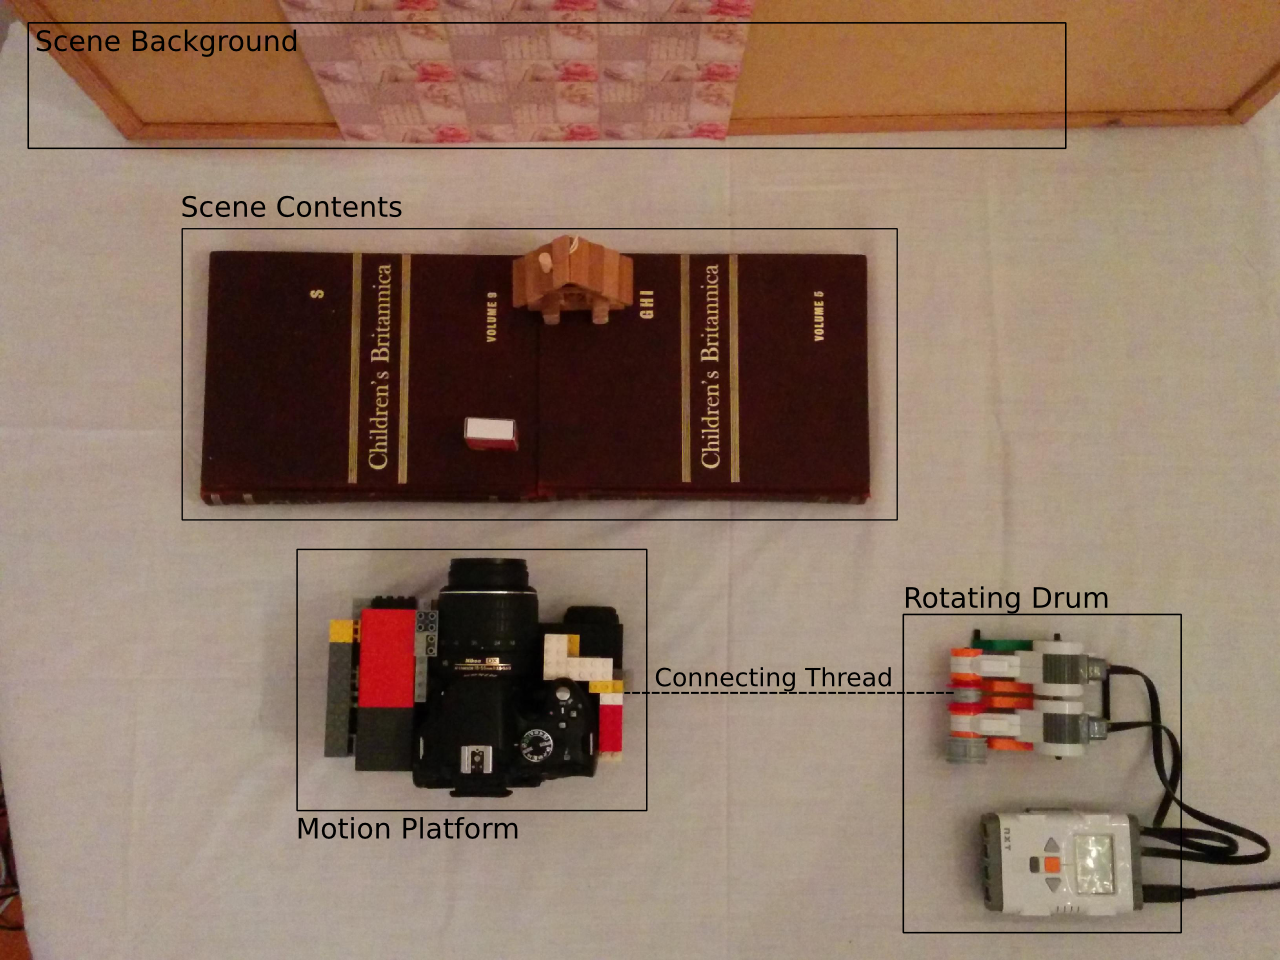
\includegraphics[width=\textwidth]{scene_contents}

\caption[Experimental scene layout]{Experimental scene layout, shown from above}
\label{fig:scene_description}

\end{figure}


\section{Image Capture}

A Lytro camera with firmware version 1.2.2 was used for the light field photography.
The Lytro camera was configured using the following settings.

\begin{table}[h]

\centering
\caption{Lytro Camera Settings}
\label{tab:lytro_settings}

\begin{tabular}{r | l}

Zoom & 1.0 \\
Creative Mode & Off \\
ND Filter & Off \\
ISO Sensitivity & Auto \\
Shutter Speed & As Required \\
Shutter Delay & 10s \\

\end{tabular}
\end{table}

The shutter delay was set to 10s to allow the motion platform to reach a stable velocity.
Once the camera countdown was started, the motion platform was commanded to move for a set distance at a set velocity.
In several cases multiple attempts were required to get the entire scene within the narrow Lytro field of view.

The captured images were transfered to an computer using the standard Lytro Desktop companion software, version 3.1.1 for Mac.
A late 2011 model Apple Mac Book Air running OSX 10.9.3 was used for image processing and version 0.2 of the Light Field Toolbox \cite{dansereau2013toolbox} was used for light field manipulation and processing in Matlab.
The image decoding, calibration and rectification process used by the LF toolbox is described in \cite{dansereau2013decoding}.

Lytro .lfp files were converted to raw image files and metadata files using the python-lfp-reader Python scripts (version 0.2) \cite{esfahbod2013python}, as per the Matlab LF Toolbox instructions.


\section{Image Processing and Deconvolution}

The raw image files were read using the Matlab LF Toolbox, and color correction applied.
The a-priori depth maps were read as images and the depth at several points in the depth map specified interactively using a graphical interface.

\hl{NEED TO TALK HERE ABOUT THE FACT THAT A-PRIORI CAMERA MOTION VELOCITY INFORMATION WAS USED, HOWEVER IN A REAL ENVIRONMENT OTHER SOURCES COULD BE USED TO GET THIS INFORMATION, E.G. THE BUILT-IN LYTRO ACCELEROMETER, OR A GPS OR OTHER SENSOR.}

A least-squares regression was then performed to find a function mapping depth map intensity to real world depth.
To reduce processing time, the depth map was then posterized into a user-specified number of 'depth planes', each with a corresponding pixel mask.
The posterization was performed by applying 1-dimensional k-means clustering to the depth map histogram, using random seed locations.
A user-specified tolerance was used to terminate the k-means operation.
\hl{Figure XXXX} shows the k-means clustering process.

\hl{[Figure XXXX goes here]}

To de-blur the light field, all possible sup-aperture slices were taken and individually de-convoled once at every scene depth using the Richardson Lucy method, as implemented in the Matlab command 'deconvlucy'.
The de-convoled sub-aperture images were then combined, using the depth plane pixel masks.
This process is described in pseudocode in \hl{Listing XXXX}.

\hl{[Listing XXXX goes here (pseudocode describing de-blurring)]}


%LF_deblurred = new_empty_lf();
%
%for i = 1 to number_of_z_planes
%    blur_length = depth_map_to_blur_length(z_plane[i])
%    psf = make_motion_psf(blur_length);
%    
%    LF_deblurred_i = new_empty_lf();
%    
%    for j = 1 to microlens_width
%        for k = 1 to microlens_height
%            subap_image = LF_blurred(j, k, :, :, :)
%            deblurred = deblur_image(subap_image, psf)
%            LF_deblurred_i(j, k, :, :, :) = deblurred
%        end
%    end
%    
%    where z_plane[i] exists:
%        copy LF_deblurred_i pixels to LF_deblurred
%end


\section{Quantitative Analysis}

Two quantitative measures were used to compare de-blurred light fields.
A 'Q-Factor' was computed to measure the reduction in image blur and the Root-Mean-Square Error (RMSE) was estimated to measure the degree of noise amplification introduced by the de-convolution.

The Q-Factor was computed by taking the central sub-aperture image from the light field and using ImageJ to manually measure the blur width in pixels of prominent straight edges within the scene.
The same edges were measured in the blurred and de-blurred images, and '\% Q increase' calculated using

\begin{equation}
Q = \frac{1}{N} \sum_{i}^{N}(1 - \frac{w_{ai}}{w_{bi}}) * 100
\end{equation}

where $i$ refers to each edge measurement, and $w_{ai}$ and $w_{bi}$ are the edge widths in pixels after and before de-blurring respectively.

The RMSE was estimated by converting the central sub-aperture image to grayscale, then selecting a small (approximately 50x50 pixel) region known to be of constant color.
The RMSE was then computed using

\begin{equation}
R = \sqrt{ \sum_{x=1}^{W} \sum_{y=1}^{H} (I(x,y) - m)^2 }
\end{equation}

Where $W$ and $H$ are the width and height of the region respectively, $I$ is the region image and $m$ is the gray level within the region.

